\documentclass[msom,dblanonrev]{informs4}
\RequirePackage{tgtermes}
\RequirePackage{newtxtext}
\RequirePackage{newtxmath}
\usepackage{booktabs}
\usepackage{tikz}
\usepackage{pgfplots}
\usepackage{fancyhdr}
\pgfplotsset{compat=1.18}
\OneAndAHalfSpacedXII

\begin{document}

\renewcommand{\thesection}{EC.\arabic{section}}
\renewcommand{\thesubsection}{\thesection.\arabic{subsection}}
\renewcommand{\thetable}{EC.\arabic{table}}
\renewcommand{\thefigure}{EC.\arabic{figure}}
\renewcommand{\theequation}{EC.\arabic{equation}}
\renewcommand{\thepage}{ec\arabic{page}}
\setcounter{page}{1}

\newcommand{\ECHeader}{%
  \footnotesize e-companion to \textbf{Anonymous}: \textit{From Forecasts to Inventory Value}%
}
\setlength{\headheight}{14pt}
\setlength{\footskip}{12pt}
\fancypagestyle{ecstyle}{%
  \fancyhf{}
  \fancyhead[L]{\ECHeader}
  \fancyhead[R]{\footnotesize\thepage}
  \renewcommand{\headrulewidth}{0.4pt}
  \renewcommand{\footrulewidth}{0pt}
}
\fancypagestyle{plain}{%
  \fancyhf{}
  \fancyhead[L]{\ECHeader}
  \fancyhead[R]{\footnotesize\thepage}
  \renewcommand{\headrulewidth}{0.4pt}
  \renewcommand{\footrulewidth}{0pt}
}
\pagestyle{ecstyle}

\RUNAUTHOR{Anonymous}
\RUNTITLE{Electronic Companion: From Forecasts to Inventory Value}
\TITLE{Electronic Companion for ``From Forecasts to Inventory Value: Time Series Foundation Models under Censored Sales''}
\ARTICLEAUTHORS{\AUTHOR{Anonymous}\AFF{}}
\date{}
\thispagestyle{ecstyle}
\vspace*{0.55in}
\begin{flushleft}
{\LARGE\bfseries Electronic Companion for ``From Forecasts to Inventory Value:\newline
Time Series Foundation Models under Censored Sales''\par}
\end{flushleft}
\vspace{1.25em}

\noindent\textbf{Companion roadmap.}
Section~EC.1 reports every point estimate and simultaneous interval from the service-level--recensoring grid.
Section~EC.2 collects the supporting decision-layer, fine-tuning, short-history, and censored-learning results.
Section~EC.3 reports the latent-demand-generator, protection-interval-dependence, PMF-reconstruction, and operational-tail-calibration checks added for distributional robustness.
The main paper's Semi-Synthetic Censoring Experiment presents the cost bridge in three consecutive steps: the exact bridge identity, arm-level total/holding/shortage costs, and component-wise two-way-bootstrap intervals.
This placement keeps the mechanism derivation adjacent to the principal $2\times2$ result, while the companion supplies the full robustness detail and grid cells used to audit it.
\vspace{1.25em}

\section{Service-Level--Recensoring Grid Results}\label{oa:grid}

Tables~\ref{tab:full_conversion} and~\ref{tab:full_mechanism} report the complete results for the $5\times 5$ service-level--recensoring grid experiment.
The conversion family contains 50 estimands ($25\;R_0+25\;R_3$) with simultaneous critical value $c_{R_0,R_3}=2.763$.
The mechanism family contains 45 estimands ($25\;A+20$ non-mechanical $\mathrm{DiD}$) with $c_{A,\mathrm{DiD}}=2.895$.
All intervals use $B=50{,}000$ two-way bootstrap resamples over SKU clusters and latent-demand draws with draw-specific SHA-256 recensoring orderings.
Throughout this section, $R_0$ and $R_3$ are relative cost effects; negative values indicate lower cost for Chronos-2 than for the retuned empirical baseline.

\begin{table}[htbp]
\centering
\caption{Full conversion-family results ($R_0$, $R_3$) across the $5\times5$ grid with pointwise 95\% confidence intervals and simultaneous 95\% upper bounds (50-dimensional max-$|t|$ correction, $c=2.763$, $B=50{,}000$). A \checkmark{} indicates that both $R_0$ and $R_3$ simultaneous upper bounds are below zero.}\label{tab:full_conversion}
\small
\resizebox{\textwidth}{!}{%
\begin{tabular}{cc rrrr rrrr c}
\toprule
 & & \multicolumn{4}{c}{$R_0$ (\%)} & \multicolumn{4}{c}{$R_3$ (\%)} & \\
\cmidrule(lr){3-6} \cmidrule(lr){7-10}
$\alpha$ & $\lambda$ & Point & CI lo & CI hi & Sim.\ hi & Point & CI lo & CI hi & Sim.\ hi & Conv.\ \\
\midrule
0.8 & 0.00 & -5.22 & -9.46 & -0.57 & +1.00 & +4.93 & +0.04 & +11.11 & +12.75 &  \\
0.8 & 0.25 & -4.49 & -8.97 & +0.63 & +2.23 & +6.60 & +1.38 & +13.27 & +15.01 &  \\
0.8 & 0.50 & -3.73 & -8.59 & +2.02 & +3.69 & +8.45 & +2.80 & +15.78 & +17.64 &  \\
0.8 & 0.75 & -2.71 & -8.10 & +3.90 & +5.70 & +10.69 & +4.49 & +18.78 & +20.83 &  \\
0.8 & 1.00 & -1.23 & -7.43 & +6.70 & +8.66 & +13.41 & +6.50 & +22.58 & +24.80 &  \\
\addlinespace
0.85 & 0.00 & -6.39 & -9.94 & -1.90 & -0.72 & +1.59 & -3.10 & +7.76 & +9.29 &  \\
0.85 & 0.25 & -5.83 & -9.62 & -0.85 & +0.38 & +3.36 & -1.83 & +10.18 & +11.86 &  \\
0.85 & 0.50 & -5.26 & -9.48 & +0.45 & +1.75 & +5.46 & -0.42 & +13.20 & +15.10 &  \\
0.85 & 0.75 & -4.50 & -9.32 & +2.22 & +3.64 & +8.17 & +1.40 & +17.12 & +19.29 &  \\
0.85 & 1.00 & -3.38 & -9.11 & +4.85 & +6.51 & +11.74 & +3.75 & +22.41 & +24.98 &  \\
\addlinespace
0.9 & 0.00 & -8.42 & -11.86 & -4.34 & -3.13 & -2.12 & -6.43 & +3.36 & +4.81 &  \\
0.9 & 0.25 & -7.93 & -11.55 & -3.52 & -2.27 & -0.36 & -5.11 & +5.73 & +7.30 &  \\
0.9 & 0.50 & -7.60 & -11.57 & -2.56 & -1.25 & +1.69 & -3.74 & +8.74 & +10.53 &  \\
0.9 & 0.75 & -7.07 & -11.55 & -1.25 & +0.19 & +4.50 & -1.81 & +12.90 & +14.92 &  \\
0.9 & 1.00 & -6.14 & -11.37 & +0.96 & +2.57 & +8.48 & +0.91 & +18.99 & +21.30 &  \\
\addlinespace
0.95 & 0.00 & -9.35 & -12.69 & -5.93 & -4.59 & -6.91 & -10.79 & -2.33 & -0.94 & \checkmark \\
0.95 & 0.25 & -9.05 & -12.50 & -5.47 & -4.12 & -5.48 & -9.60 & -0.47 & +0.98 &  \\
0.95 & 0.50 & -8.97 & -12.71 & -5.00 & -3.56 & -3.78 & -8.40 & +2.05 & +3.63 &  \\
0.95 & 0.75 & -8.76 & -12.94 & -4.27 & -2.66 & -1.24 & -6.64 & +5.90 & +7.66 &  \\
0.95 & 1.00 & -8.35 & -13.36 & -2.99 & -1.10 & +2.71 & -3.94 & +12.45 & +14.43 &  \\
\addlinespace
0.98 & 0.00 & -12.55 & -17.14 & -7.82 & -5.94 & -13.02 & -17.83 & -7.70 & -5.83 & \checkmark \\
0.98 & 0.25 & -12.59 & -17.44 & -7.57 & -5.61 & -12.18 & -17.21 & -6.48 & -4.54 & \checkmark \\
0.98 & 0.50 & -12.97 & -18.30 & -7.41 & -5.23 & -11.15 & -16.61 & -4.81 & -2.66 & \checkmark \\
0.98 & 0.75 & -13.39 & -19.55 & -7.09 & -4.55 & -9.45 & -15.65 & -2.09 & +0.39 &  \\
0.98 & 1.00 & -13.91 & -21.80 & -6.49 & -3.10 & -6.49 & -13.94 & +3.20 & +6.12 &  \\
\bottomrule
\end{tabular}
}
\end{table}

\begin{table}[htbp]
\centering
\caption{Full mechanism-family results ($A$, $\mathrm{DiD}$) across the $5\times5$ grid with simultaneous 95\% confidence intervals (45-dimensional max-$|t|$ correction, $c=2.895$, $B=50{,}000$). $\mathrm{DiD}(\alpha,0)\equiv0$ by construction (\textdagger). Bold entries have simultaneous intervals excluding zero.}\label{tab:full_mechanism}
\small
\begin{tabular}{cc rrr rrr}
\toprule
 & & \multicolumn{3}{c}{$A$ (\%)} & \multicolumn{3}{c}{$\mathrm{DiD}$ (\%)} \\
\cmidrule(lr){3-5} \cmidrule(lr){6-8}
$\alpha$ & $\lambda$ & Point & Sim.\ lo & Sim.\ hi & Point & Sim.\ lo & Sim.\ hi \\
\midrule
0.8 & 0.00 & \textbf{+10.16} & +4.16 & +16.15 & 0\textsuperscript{\textdagger} & --- & --- \\
0.8 & 0.25 & \textbf{+11.09} & +4.64 & +17.54 & \textbf{-0.93} & -1.66 & -0.20 \\
0.8 & 0.50 & \textbf{+12.18} & +5.14 & +19.22 & \textbf{-2.03} & -3.64 & -0.41 \\
0.8 & 0.75 & \textbf{+13.40} & +5.62 & +21.17 & \textbf{-3.24} & -5.94 & -0.55 \\
0.8 & 1.00 & \textbf{+14.64} & +5.89 & +23.40 & \textbf{-4.49} & -8.62 & -0.35 \\
\addlinespace
0.85 & 0.00 & \textbf{+7.98} & +2.80 & +13.17 & 0\textsuperscript{\textdagger} & --- & --- \\
0.85 & 0.25 & \textbf{+9.19} & +3.50 & +14.87 & \textbf{-1.20} & -1.97 & -0.44 \\
0.85 & 0.50 & \textbf{+10.72} & +4.34 & +17.10 & \textbf{-2.74} & -4.47 & -1.01 \\
0.85 & 0.75 & \textbf{+12.67} & +5.34 & +20.00 & \textbf{-4.69} & -7.71 & -1.67 \\
0.85 & 1.00 & \textbf{+15.13} & +6.42 & +23.83 & \textbf{-7.14} & -11.95 & -2.34 \\
\addlinespace
0.9 & 0.00 & \textbf{+6.30} & +1.71 & +10.90 & 0\textsuperscript{\textdagger} & --- & --- \\
0.9 & 0.25 & \textbf{+7.57} & +2.40 & +12.75 & \textbf{-1.27} & -2.14 & -0.40 \\
0.9 & 0.50 & \textbf{+9.29} & +3.27 & +15.32 & \textbf{-2.99} & -5.00 & -0.98 \\
0.9 & 0.75 & \textbf{+11.57} & +4.25 & +18.90 & \textbf{-5.27} & -8.92 & -1.62 \\
0.9 & 1.00 & \textbf{+14.62} & +5.23 & +24.01 & \textbf{-8.32} & -14.44 & -2.19 \\
\addlinespace
0.95 & 0.00 & +2.44 & -1.82 & +6.70 & 0\textsuperscript{\textdagger} & --- & --- \\
0.95 & 0.25 & +3.58 & -1.34 & +8.49 & \textbf{-1.14} & -2.12 & -0.15 \\
0.95 & 0.50 & +5.20 & -0.76 & +11.15 & \textbf{-2.76} & -5.08 & -0.43 \\
0.95 & 0.75 & +7.51 & -0.21 & +15.24 & \textbf{-5.07} & -9.55 & -0.60 \\
0.95 & 1.00 & +11.06 & -0.06 & +22.18 & \textbf{-8.62} & -16.95 & -0.30 \\
\addlinespace
0.98 & 0.00 & -0.47 & -4.36 & +3.41 & 0\textsuperscript{\textdagger} & --- & --- \\
0.98 & 0.25 & +0.41 & -4.03 & +4.85 & -0.89 & -1.84 & +0.07 \\
0.98 & 0.50 & +1.82 & -3.66 & +7.30 & -2.29 & -4.68 & +0.09 \\
0.98 & 0.75 & +3.94 & -3.53 & +11.41 & -4.41 & -9.26 & +0.43 \\
0.98 & 1.00 & +7.42 & -4.61 & +19.45 & -7.89 & -17.82 & +2.03 \\
\bottomrule
\end{tabular}
\end{table}

\clearpage
\section{Supporting Static Decision-Layer Results}\label{oa:static}

\begin{table}[htbp]
\caption{Ablation of the hybrid pipeline's three components, evaluated on validation and test windows ($\alpha=0.85$). Each row adds one component cumulatively. $\Delta$\% is relative to GBDT-lean.}\label{tab:oa_ablation}
\centering\small
\begin{tabular}{lccc cc cc}
\toprule
 & & & & \multicolumn{2}{c}{\textbf{Validation}} & \multicolumn{2}{c}{\textbf{Test}} \\
\cmidrule(lr){5-6}\cmidrule(lr){7-8}
\textbf{Configuration} & \textbf{E2E} & \textbf{Rich} & \textbf{TSFM} & \textbf{Cost} & \textbf{$\Delta$\%} & \textbf{Cost} & \textbf{$\Delta$\%} \\
\midrule
\multicolumn{8}{l}{\emph{GBDT decision model}} \\
GBDT-lean            &     &     &     & 0.674 & ---    & 0.385 & ---    \\
ERM-GBDT-lean        & \checkmark &     &     & 0.605 & $-$10\% & 0.358 & $-$7\%  \\
ERM-GBDT-rich        & \checkmark & \checkmark &     & 0.509 & $-$24\% & 0.298 & $-$23\% \\
Hybrid-GBDT          & \checkmark & \checkmark & \checkmark & 0.495 & $-$27\% & 0.286 & $-$26\% \\
\midrule
\multicolumn{8}{l}{\emph{Linear decision model}} \\
ERM-linear-lean      & \checkmark &     &     & 0.611 & $-$9\%  & 0.419 & $+$9\%  \\
ERM-linear-rich      & \checkmark & \checkmark &     & 0.462 & $-$31\% & 0.329 & $-$15\% \\
Hybrid-linear        & \checkmark & \checkmark & \checkmark & 0.455 & $-$33\% & 0.291 & $-$24\% \\
\midrule
\multicolumn{8}{l}{\emph{Reference: history-only TSFM}} \\
Chronos-2-FT         &     &     &     & 0.549 & $-$19\% & 0.310 & $-$19\% \\
\bottomrule
\end{tabular}
\end{table}

\begin{table}[htbp]
\caption{Illustrative annualized economic impact relative to the empirical baseline ($\alpha=0.85$, $\kappa_h=0.20$, $L=1$ day). Annual figures scale the measured per-SKU-month delta to a 28{,}626-SKU portfolio.}\label{tab:oa_annualized}
\centering\small
\resizebox{\textwidth}{!}{%
\begin{tabular}{lcccc}
\toprule
\textbf{Model} & \textbf{Cost/SKU-month} & $\boldsymbol{\Delta}$\textbf{/SKU-month} & $\boldsymbol{\Delta}$\textbf{\%} & \textbf{Annual} $\boldsymbol{\Delta}$ \\
\midrule
Chronos-2 (fine-tuned) & \$41.09 & $-$\$4.38 & $-$9.6\% & $-$\$1.50M \\
Chronos-2 (zero-shot)  & \$41.57 & $-$\$3.90 & $-$8.6\% & $-$\$1.34M \\
GBDT (lean)            & \$53.71 & $+$\$8.24 & $+$18.1\% & $+$\$2.83M \\
\bottomrule
\end{tabular}
}
\end{table}

\begin{table}[htbp]
\caption{Operating-point fine-tuning: newsvendor cost by loss variant and lead time ($\alpha=0.85$, July 2019).}\label{tab:oa_ws3}
\centering\small
\begin{tabular}{lccc}
\toprule
& \multicolumn{3}{c}{\textbf{Lead time $L$ (days)}} \\
\cmidrule(lr){2-4}
\textbf{Loss variant} & $L=1$ & $L=7$ & $L=14$ \\
\midrule
Chronos-2 (zero-shot) & 18.72 & 16.61 & 16.81 \\
Pinball (standard ft) & 18.56 & 16.00 & 15.45 \\
Operating-point loss  & 17.98 & 15.33 & 14.65 \\
Focused pinball       & 18.29 & 15.84 & 15.47 \\
Empirical quantile    & 20.51 & 17.77 & 16.71 \\
\bottomrule
\end{tabular}
\end{table}

\begin{table}[htbp]
\caption{Chronos-2 performance by context length (July 2019, $n=442$ short-history-eligible SKUs).}\label{tab:oa_context}
\centering\small
\begin{tabular}{lcccc}
\toprule
\textbf{Context} & \textbf{NPL} & \textbf{Cost} & \textbf{CSR} & \textbf{FR} \\
\midrule
7 days   & 0.916 & 134.58 & 0.993 & 0.803 \\
14 days  & 0.320 & 106.59 & 0.975 & 0.783 \\
30 days  & 0.271 & 94.20  & 0.962 & 0.774 \\
60 days  & 0.266 & 90.91  & 0.939 & 0.763 \\
90 days  & 0.265 & 90.61  & 0.921 & 0.755 \\
Full     & 0.262 & 90.59  & 0.921 & 0.749 \\
\midrule
Empirical (full) & 0.332 & 101.37 & 0.878 & 0.662 \\
\bottomrule
\end{tabular}
\end{table}

\begin{table}[htbp]
\caption{Comparison with DDM on the Zhao validation window ($\alpha=0.85$, $L=1$ day).}\label{tab:oa_ddm}
\centering\small
\begin{tabular}{lcccc}
\toprule
\textbf{Model} & \textbf{Cost (Jul)} & \textbf{Cost (Aug)} & \textbf{CSR} & \textbf{$S$ (median)} \\
\midrule
Chronos-2 (zero-shot) & 18.72 & 63.11 & 0.921 & 19.5 \\
Empirical quantile    & 20.51 & 69.00 & 0.893 & 16.0 \\
DDM                   & 35.95 & 78.87 & 0.975 & 60.5 \\
\bottomrule
\end{tabular}
\end{table}

\begin{figure}[htbp]
\centering
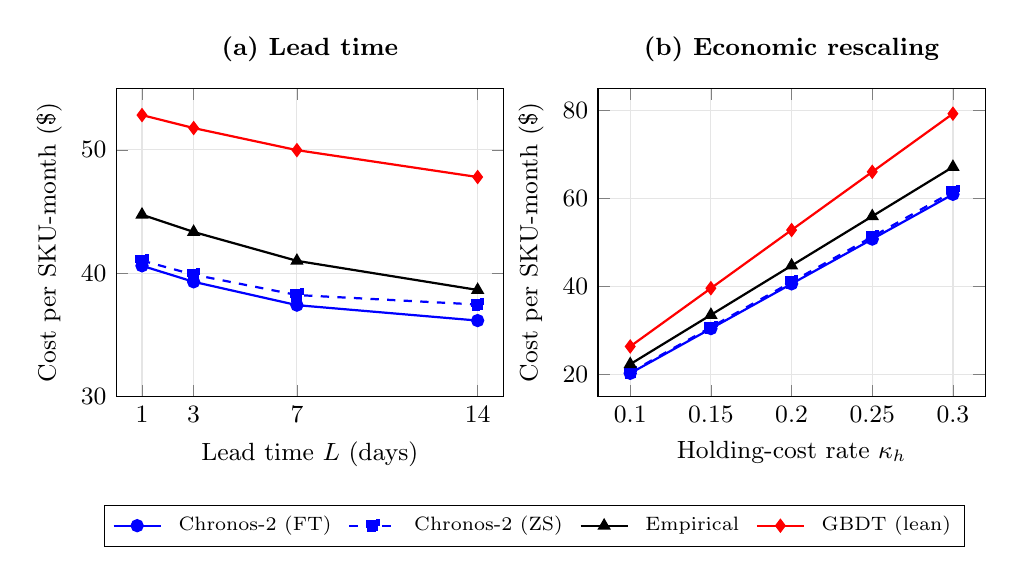
\begin{tikzpicture}
\begin{axis}[
    name=left, width=6.5cm, height=5.5cm,
    xlabel={Lead time $L$ (days)}, ylabel={Cost per SKU-month (\$)},
    xtick={1,3,7,14}, xmin=0, xmax=15, ymin=30, ymax=55,
    legend style={at={(1.08,-0.35)}, anchor=north, font=\scriptsize, legend columns=4, column sep=4pt},
    grid=major, grid style={gray!20}, tick label style={font=\small}, label style={font=\small},
    title style={font=\small\bfseries}, title={(a) Lead time}, mark size=2pt]
\addplot[blue, thick, mark=*] coordinates {(1,40.61) (3,39.31) (7,37.42) (14,36.17)};
\addplot[blue, thick, mark=square*, dashed] coordinates {(1,41.03) (3,39.89) (7,38.24) (14,37.47)};
\addplot[black, thick, mark=triangle*] coordinates {(1,44.75) (3,43.35) (7,41.01) (14,38.65)};
\addplot[red, thick, mark=diamond*] coordinates {(1,52.82) (3,51.77) (7,49.98) (14,47.80)};
\legend{Chronos-2 (FT), Chronos-2 (ZS), Empirical, GBDT (lean)}
\end{axis}
\begin{axis}[
    at={(left.east)}, anchor=west, xshift=1.2cm,
    width=6.5cm, height=5.5cm,
    xlabel={Holding-cost rate $\kappa_h$}, ylabel={Cost per SKU-month (\$)},
    xtick={0.10,0.15,0.20,0.25,0.30}, xmin=0.08, xmax=0.32, ymin=15, ymax=85,
    grid=major, grid style={gray!20}, tick label style={font=\small}, label style={font=\small},
    title style={font=\small\bfseries}, title={(b) Economic rescaling}, mark size=2pt]
\addplot[blue, thick, mark=*] coordinates {(0.10,20.31) (0.15,30.46) (0.20,40.61) (0.25,50.76) (0.30,60.92)};
\addplot[blue, thick, mark=square*, dashed] coordinates {(0.10,20.52) (0.15,30.77) (0.20,41.03) (0.25,51.29) (0.30,61.55)};
\addplot[black, thick, mark=triangle*] coordinates {(0.10,22.38) (0.15,33.56) (0.20,44.75) (0.25,55.94) (0.30,67.13)};
\addplot[red, thick, mark=diamond*] coordinates {(0.10,26.41) (0.15,39.61) (0.20,52.82) (0.25,66.02) (0.30,79.22)};
\end{axis}
\end{tikzpicture}
\caption{Static newsvendor cost across economic parameters ($\alpha=0.85$). At fixed $\alpha$, panel (b) scales $h$ and $p$ proportionally and is an economic rescaling rather than an independent robustness test.}\label{fig:oa_sensitivity}
\end{figure}

\begin{figure}[htbp]
\centering
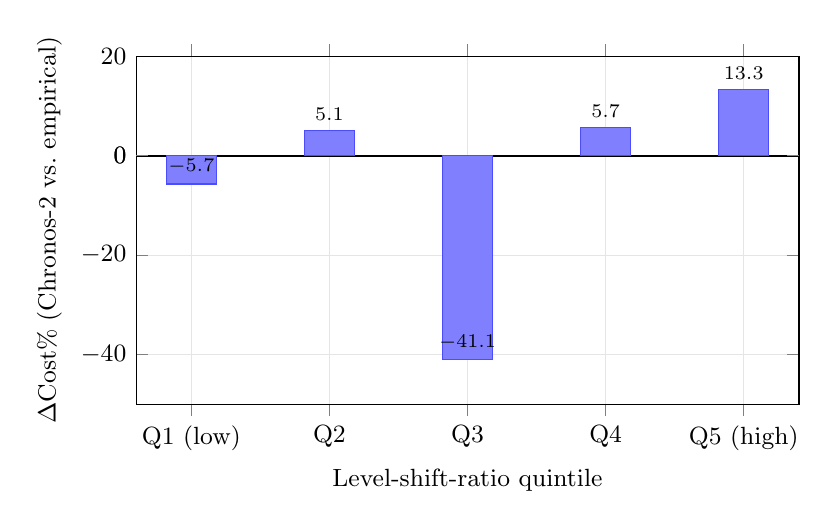
\begin{tikzpicture}
\begin{axis}[
    ybar, width=10cm, height=6cm,
    xlabel={Level-shift-ratio quintile},
    ylabel={$\Delta$Cost\% (Chronos-2 vs.\ empirical)},
    symbolic x coords={Q1 (low), Q2, Q3, Q4, Q5 (high)}, xtick=data,
    ymin=-50, ymax=20, bar width=18pt, nodes near coords,
    nodes near coords style={font=\scriptsize, anchor=south},
    every node near coord/.append style={/pgf/number format/.cd, fixed, fixed zerofill, precision=1, /tikz/.cd},
    grid=major, grid style={gray!20}, tick label style={font=\small}, label style={font=\small},
    extra y ticks={0}, extra y tick style={grid=major, grid style={black, thick}}]
\addplot[fill=blue!50, draw=blue!70] coordinates {
  (Q1 (low), -5.7) (Q2, 5.1) (Q3, -41.1) (Q4, 5.7) (Q5 (high), 13.3)
};
\end{axis}
\end{tikzpicture}
\caption{Cost difference by level-shift-ratio quintile. Positive = Chronos-2 cheaper. $n\approx674$ per quintile. Q5 contains the largest upward shifts and shows the strongest advantage ($+13.3\%$); the Q3 aggregate is driven by three large-error SKU-months.}\label{fig:oa_shift}
\end{figure}

\begin{figure}[htbp]
\centering
\resizebox{\textwidth}{!}{%
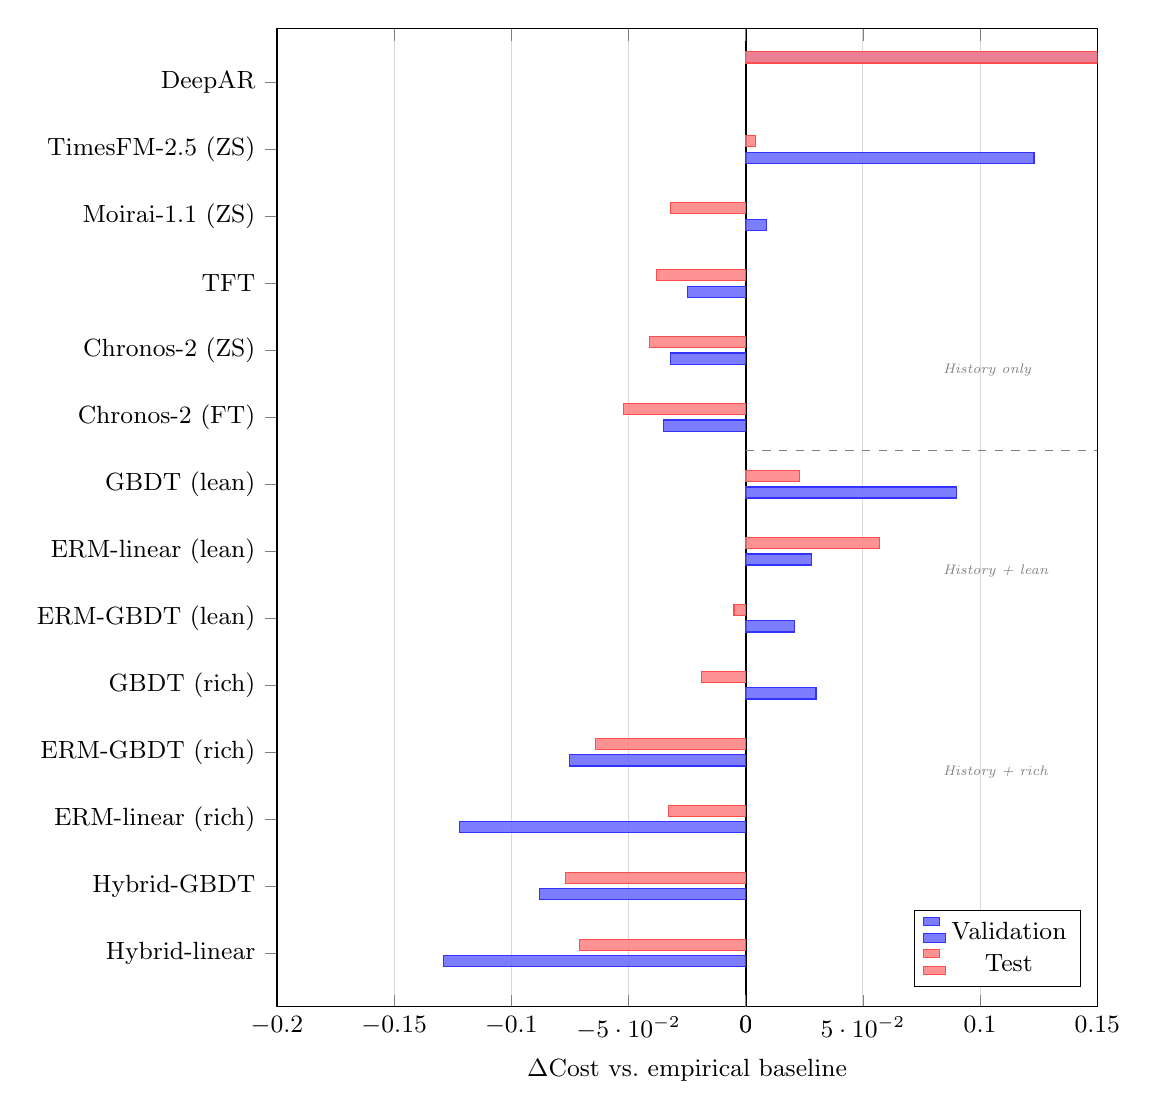
\begin{tikzpicture}
\begin{axis}[
    xbar, width=12cm, height=14cm,
    xlabel={$\Delta$Cost vs.\ empirical baseline}, xmin=-0.20, xmax=0.15,
    ytick={1,2,3,4,5,6,7,8,9,10,11,12,13,14},
    yticklabels={{DeepAR},{TimesFM-2.5 (ZS)},{Moirai-1.1 (ZS)},{TFT},{Chronos-2 (ZS)},{Chronos-2 (FT)},{GBDT (lean)},{ERM-linear (lean)},{ERM-GBDT (lean)},{GBDT (rich)},{ERM-GBDT (rich)},{ERM-linear (rich)},{Hybrid-GBDT},{Hybrid-linear}},
    y dir=reverse, ytick pos=left,
    legend style={at={(0.98,0.02)}, anchor=south east, font=\small},
    bar width=4pt, xmajorgrids=true, grid style={gray!30},
    extra x ticks={0}, extra x tick style={grid=major, grid style={black, thick}},
    tick label style={font=\small}, label style={font=\small},
    every axis plot/.append style={fill opacity=0.85}, ymin=0.2, ymax=14.8]
\addplot[fill=blue!60, draw=blue!80] coordinates {
  (-0.129,14) (-0.088,13) (-0.122,12) (-0.075,11) (0.030,10) (0.021,9) (0.028,8) (0.090,7) (-0.035,6) (-0.032,5) (-0.025,4) (0.009,3) (0.123,2)
};
\addplot[fill=red!50, draw=red!70] coordinates {
  (-0.071,14) (-0.077,13) (-0.033,12) (-0.064,11) (-0.019,10) (-0.005,9) (0.057,8) (0.023,7) (-0.052,6) (-0.041,5) (-0.038,4) (-0.032,3) (0.004,2)
};
\addplot[fill=blue!60, draw=blue!80, forget plot] coordinates {(0.317,1)};
\addplot[fill=red!50, draw=red!70, forget plot] coordinates {(0.195,1)};
\legend{Validation, Test}
\draw[dashed, gray] (axis cs:0,6.5) -- (axis cs:0.15,6.5);
\node[anchor=west, font=\tiny\itshape, gray] at (axis cs:0.08,14.3) {TSFM + rich};
\node[anchor=west, font=\tiny\itshape, gray] at (axis cs:0.08,11.3) {History + rich};
\node[anchor=west, font=\tiny\itshape, gray] at (axis cs:0.08,8.3) {History + lean};
\node[anchor=west, font=\tiny\itshape, gray] at (axis cs:0.08,5.3) {History only};
\end{axis}
\end{tikzpicture}
}
\caption{Decision-layer $\Delta$Cost relative to the empirical baseline ($\alpha=0.85$, $L=1$, $\kappa_h=0.20$). Negative values indicate cost savings. DeepAR bars are truncated (validation: $+0.317$; test: $+0.195$).}\label{fig:oa_layerc}
\end{figure}

\clearpage
\section{Distributional Robustness and Tail Calibration}\label{oa:distribution}

This section reports the checks that support the semi-synthetic and protection-interval constructions in the main paper.
All analyses retain the same 1{,}135 cost-eligible series, five scored origins, two high service levels, origin-specific retuned empirical comparators, and fixed policy support.
The exact cost-bridge identity, arm-level total/holding/shortage costs, and component-wise bridge intervals are grouped together in the main paper's ``Semi-Synthetic Censoring Experiment'' subsection (Tables ``Arm-level dynamic-cost bridge'' and ``Holding/shortage decomposition'').

\subsection{Latent-Demand Generator Sensitivity}\label{oa:dgp}

The baseline empirical-conditional generator classifies a series--origin month as censored when monthly logged sales weakly exceed positive beginning inventory.
For each series, it forms a donor distribution from daily sales in origin months not so classified and, on each positive-sales day in a classified month, draws from that empirical distribution conditional on the draw being at least the logged sale.
An empty conditional donor set invokes the geometric-excess fallback described in the main paper.

Two parametric generators use the same classified months and imputed days.
Let $\widehat\mu_i$ and $\widehat v_i$ be the mean and sample variance of series $i$'s daily sales in nonclassified origin months.
The Poisson generator draws
\[
X_{it}\sim \operatorname{Poisson}(\widehat\mu_i)\mid X_{it}\geq Y_{it}.
\]
When $\widehat v_i>\widehat\mu_i$, the negative-binomial generator uses
\[
r_i=\frac{\widehat\mu_i^2}{\widehat v_i-\widehat\mu_i},
\qquad
q_i=\frac{r_i}{r_i+\widehat\mu_i},
\qquad
X_{it}\sim \operatorname{NB}(r_i,q_i)\mid X_{it}\geq Y_{it};
\]
otherwise it uses the Poisson specification.
Numerically degenerate truncations use the same series-specific geometric fallback.
All three generators leave every other day equal to logged sales and use 50 SHA-256-keyed draws.

Table~\ref{tab:oa_dgp_diag} summarizes positive imputed increments, $D-Y>0$.
The three specifications span a transparent severity range: Poisson has the lightest positive excess, the moment-matched negative binomial is intermediate, and empirical conditional resampling has the largest mean and upper tail.

\begin{table}[htbp]
\caption{Latent-demand-generator diagnostics. Counts and moments are computed over draw--day--series observations with a strictly positive imputed increment $D-Y$.}\label{tab:oa_dgp_diag}
\centering\small
\begin{tabular}{lrrrr}
\toprule
\textbf{Generator} & \textbf{Positive increments} & \textbf{Mean} & \textbf{Median} & \textbf{95th pct.} \\
\midrule
Empirical conditional & 1{,}731{,}518 & 6.33 & 2 & 22 \\
Poisson               &   691{,}442 & 2.79 & 1 & 8 \\
Negative binomial     &   988{,}685 & 5.03 & 2 & 16 \\
\bottomrule
\end{tabular}
\end{table}

\begin{table}[htbp]
\caption{Latent-demand-generator sensitivity. Relative effects are percentages; attenuation and DiD are percentage points. Brackets report 95\% intervals from 10{,}000 two-way bootstrap resamples (SKU clusters $\times$ latent-demand draws).}\label{tab:oa_dgp_effects}
\centering\small
\resizebox{\textwidth}{!}{%
\begin{tabular}{lrrrr}
\toprule
\textbf{Generator} & $\boldsymbol{R_D}$ \textbf{static} & $\boldsymbol{R_D}$ \textbf{dynamic} & $\boldsymbol{A_D}$ & \textbf{DiD} \\
\midrule
Empirical conditional & $-11.59\;[-15.72,-7.35]$ & $-11.12\;[-15.65,-6.15]$ & $+0.47\;[-1.81,+3.65]$ & $-8.28\;[-17.22,-4.23]$ \\
Poisson               & $-13.15\;[-19.29,-7.09]$ & $-6.94\;[-13.17,+1.41]$  & $+6.21\;[+1.90,+14.58]$ & $-2.54\;[-5.59,-1.14]$ \\
Negative binomial     & $-12.51\;[-17.66,-7.15]$ & $-9.79\;[-15.39,-3.03]$  & $+2.72\;[-0.17,+7.45]$  & $-6.03\;[-13.49,-2.80]$ \\
\bottomrule
\end{tabular}
}
\end{table}

The DiD is negative with an interval below zero for every generator.
Its magnitude follows the recovered-excess severity in Table~\ref{tab:oa_dgp_diag}: 2.54 percentage points for Poisson, 6.03 for negative binomial, and 8.28 for empirical conditional resampling.
The dynamic effect remains statistically detectable under the empirical and negative-binomial generators; the lighter Poisson generator yields a negative point estimate with an interval spanning zero.

\subsection{PMF Reconstruction and Protection-Interval Dependence}\label{oa:aggregation}

The baseline PMF maps the repaired 21-point quantile grid to the integer support by taking the midpoint of the lower and upper CDF bounds implied at each support point.
The first reconstruction check instead linearly interpolates the repaired inverse quantile function between adjacent quantile levels and numerically inverts it on the integer support.
The second retains midpoint reconstruction but uses the 12 levels
\[
\{0.01,0.10,0.20,0.30,0.40,0.50,0.60,0.70,0.80,0.90,0.95,0.99\}.
\]

The dependence checks preserve these daily marginal CDFs and generate protection-interval demand through a Gaussian-copula AR(1) design.
For independent scrambled Sobol normal scores $\epsilon_t$, we set
\[
Z_1=\epsilon_1,
\qquad
Z_t=\rho Z_{t-1}+\sqrt{1-\rho^2}\,\epsilon_t,
\qquad
U_t=\Phi(Z_t),
\]
and obtain daily integer demand by applying each forecast CDF's inverse to $U_t$.
The stocking target is the empirical $\alpha$ quantile of 16{,}384 simulated protection-interval sums.
The stress values $\rho=0.25$ and $0.50$ are applied identically to every arm.

\begin{table}[htbp]
\caption{PMF-reconstruction and protection-interval-dependence sensitivity. Relative effects are percentages; attenuation is in percentage points. Brackets report 95\% SKU-cluster-bootstrap intervals ($B=10{,}000$).}\label{tab:oa_aggregation}
\centering\scriptsize
\resizebox{\textwidth}{!}{%
\begin{tabular}{llrrr}
\toprule
\textbf{Construction} & $\boldsymbol{\alpha}$ & $\boldsymbol{R_0}$ & $\boldsymbol{R_3}$ & \textbf{Attenuation} \\
\midrule
Midpoint-21 (baseline) & Pooled & $-12.21\;[-18.86,-5.68]$ & $-3.46\;[-10.73,+6.50]$ & $+8.75\;[+3.39,+19.58]$ \\
 & 0.95 & $-8.35\;[-13.28,-2.96]$ & $+2.71\;[-4.01,+12.62]$ & $+11.06\;[+5.62,+20.75]$ \\
 & 0.98 & $-13.91\;[-21.72,-6.36]$ & $-6.50\;[-14.10,+3.34]$ & $+7.42\;[+2.16,+18.34]$ \\
\addlinespace
Inverse-quantile-linear-21 & Pooled & $-11.06\;[-17.65,-3.88]$ & $-2.31\;[-9.96,+8.50]$ & $+8.75\;[+3.48,+19.74]$ \\
 & 0.95 & $-7.06\;[-11.82,-1.22]$ & $+4.20\;[-2.78,+14.79]$ & $+11.25\;[+6.05,+20.62]$ \\
 & 0.98 & $-12.83\;[-20.65,-4.53]$ & $-5.54\;[-13.51,+5.18]$ & $+7.30\;[+2.09,+18.55]$ \\
\addlinespace
Midpoint-12 & Pooled & $-12.20\;[-18.86,-5.72]$ & $-3.36\;[-10.64,+6.65]$ & $+8.84\;[+3.38,+19.79]$ \\
 & 0.95 & $-8.07\;[-12.98,-2.68]$ & $+3.07\;[-3.69,+13.15]$ & $+11.14\;[+5.59,+21.03]$ \\
 & 0.98 & $-14.01\;[-21.83,-6.51]$ & $-6.51\;[-14.11,+3.34]$ & $+7.50\;[+2.17,+18.56]$ \\
\addlinespace
AR(1) copula, $\rho=0.25$ & Pooled & $-11.17\;[-17.79,-3.97]$ & $-1.61\;[-9.73,+10.20]$ & $+9.56\;[+3.88,+21.38]$ \\
 & 0.95 & $-7.24\;[-12.21,-1.34]$ & $+4.96\;[-2.46,+16.30]$ & $+12.20\;[+6.43,+22.54]$ \\
 & 0.98 & $-12.93\;[-20.68,-4.58]$ & $-4.89\;[-13.38,+6.76]$ & $+8.05\;[+2.52,+20.20]$ \\
\addlinespace
AR(1) copula, $\rho=0.50$ & Pooled & $-9.55\;[-16.39,-1.73]$ & $+2.15\;[-7.41,+17.09]$ & $+11.70\;[+5.30,+25.55]$ \\
 & 0.95 & $-5.40\;[-10.64,+1.90]$ & $+8.76\;[-0.06,+22.66]$ & $+14.16\;[+7.98,+25.21]$ \\
 & 0.98 & $-11.46\;[-19.25,-2.70]$ & $-1.24\;[-11.12,+13.81]$ & $+10.22\;[+3.84,+25.08]$ \\
\bottomrule
\end{tabular}
}
\end{table}

Both alternative PMF reconstructions reproduce the baseline attenuation to within 0.1 percentage point in the pooled estimate.
Positive temporal dependence produces a different and economically interpretable shift: the static effect continues to favor Chronos-2, while attenuation increases with $\rho$ and the dynamic point estimate weakens.

\subsection{Operational Tail-Calibration Diagnostics}\label{oa:tailcal}

For demand measure $e\in\{Y,D\}$, policy $m$, and service level $\alpha$, define operational coverage and mean excess units as
\[
\operatorname{Cov}_{m,e,\alpha}
=\Pr\!\left(D^{e}_{io}\leq S_{m,io,\alpha}\right),
\qquad
\operatorname{Exc}_{m,e,\alpha}
=\mathbb E\!\left(D^{e}_{io}-S_{m,io,\alpha}\right)^+,
\]
where $D^{e}_{io}$ is realized protection-interval demand and $S_{m,io,\alpha}$ is the fixed policy target.
Coverage gap is $\operatorname{Cov}_{m,e,\alpha}-\alpha$, and exceedance rate is one minus coverage.

\begin{table}[htbp]
\caption{Operational tail calibration. Coverage, gap, and exceedance are percentages; mean excess units average $(D-S)^+$ over all scored cells. Logged-sales intervals resample SKU clusters; latent-demand intervals use the two-way SKU-cluster $\times$ draw bootstrap ($B=10{,}000$).}\label{tab:oa_tailcal}
\centering\scriptsize
\resizebox{\textwidth}{!}{%
\begin{tabular}{llcrrrr}
\toprule
\textbf{Demand} & \textbf{Policy} & $\boldsymbol{\alpha}$ & \textbf{Coverage} & \textbf{Gap [95\% CI]} & \textbf{Exceedance} & \textbf{Mean excess [95\% CI]} \\
\midrule
$Y$ & Chronos-2 & 0.95 & 88.25 & $-6.75\;[-7.65,-5.89]$ & 11.75 & $7.85\;[4.67,12.18]$ \\
$Y$ & Emp-retuned & 0.95 & 84.14 & $-10.86\;[-11.83,-9.91]$ & 15.86 & $9.04\;[5.72,13.48]$ \\
$Y$ & Chronos-2 & 0.98 & 90.87 & $-7.13\;[-7.94,-6.35]$ & 9.13 & $7.11\;[4.00,11.40]$ \\
$Y$ & Emp-retuned & 0.98 & 87.24 & $-10.76\;[-11.69,-9.84]$ & 12.76 & $8.49\;[5.17,12.86]$ \\
\addlinespace
$D$ & Chronos-2 & 0.95 & 76.82 & $-18.18\;[-19.64,-16.72]$ & 23.18 & $24.79\;[17.64,34.00]$ \\
$D$ & Emp-retuned & 0.95 & 72.57 & $-22.43\;[-23.90,-20.94]$ & 27.43 & $27.25\;[19.82,36.50]$ \\
$D$ & Chronos-2 & 0.98 & 80.34 & $-17.66\;[-19.03,-16.31]$ & 19.66 & $22.81\;[15.83,31.86]$ \\
$D$ & Emp-retuned & 0.98 & 76.53 & $-21.47\;[-22.91,-20.01]$ & 23.47 & $25.53\;[18.22,34.69]$ \\
\bottomrule
\end{tabular}
}
\end{table}

Chronos-2 has higher operational coverage and lower mean excess units in every demand--service-level cell.
The coverage difference relative to Emp-retuned ranges from 3.63 to 4.25 percentage points and is similar under logged sales and latent demand.
These policy-level diagnostics complement aggregate pinball loss by evaluating the tail events that enter shortage exposure directly.

\paragraph{Reproduction.}
The script \texttt{src/f2d/run\_review\_robustness.py} produces Tables~\ref{tab:oa_dgp_diag}--\ref{tab:oa_tailcal} without modifying the frozen principal outputs.
The reported run uses 50 latent-demand draws, 16{,}384 scrambled Sobol paths, and 10{,}000 bootstrap replications; the repository README records the complete command and pinned model revision.

\end{document}
